\section{Remote Attestation}
\label{ch:remote-attestation}

Running applications inside a CC enabled environment is not enough in order to
deepen the trust with clients or third-parties. In order to prove that the
application is running inside a CC enabled environment and that neither the
application nor the system it is running on has been tampered with, the service
provider can facilitate remote attestation.

In a remote attestation environment there are at least two roles: the attester
and the relying party. The attester produces information about itself
(evidence), on which the relying party makes a decision whether to trust the
attester or not. In our context the attester would be the system running a
client application and the relying party would be the client accessing or
sending data to the application.

\subsection{Remote Attestation Procedures (RATS)}
\label{sec:rats}

\begin{figure}
  \centering
  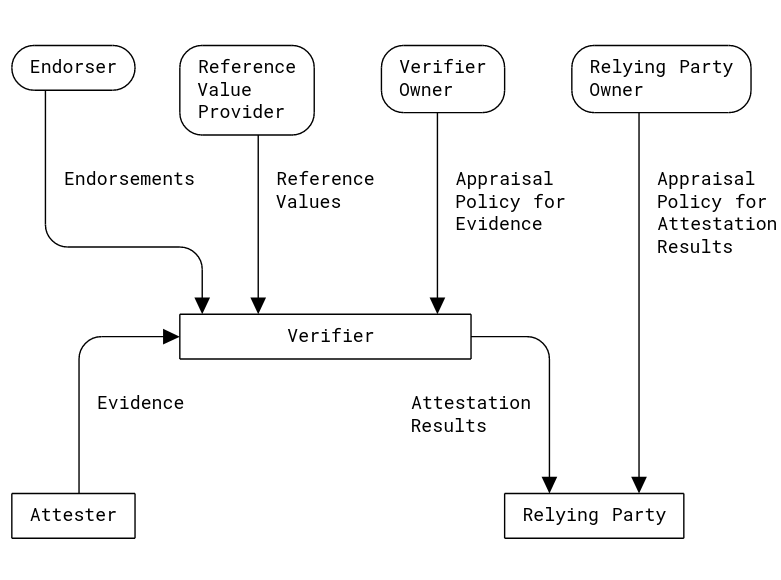
\includegraphics[width=0.7\linewidth]{resources/rats-architecture.png}
  \caption[RATS architectural overview]{
    RATS architectural overview.\\
    Source: \citetitle{rfc9334} \cite{rfc9334}
  }
  \label{figure:rats-architecture}
\end{figure}

Remote Attestation Procedures (RATS) defines a general architecture, roles, and
messages in order to establish trust between the relying party and the attester.
Figure \ref{figure:rats-architecture} shows the general architecture. RATS
introduces few new roles where the most prominent one is the verifier. It
produces attestation results by using evidence, endorsements, reference values,
and applying an appraisal policy to assess the trustworthiness of the attester.
This procedure is called ``appraisal of evidence''. These attestation results
then support the decision process of the relying party on whether to trust the
attester or not.

\todo[inline]{RATS Architecture - indepth}
